\chapter{\uppercase{Modified Interior Penalty on Arbitrary Polygonal Cells}}
\label{mip_chapter}
\section{Introduction}
In Chapter \ref{anmg_chapter}, we noted that at the coarsest level of ANMG 
a Diffusion Synthetic Acceleration needs to be solved. 
Because analytical and closed form solutions are unavailable for most
radiation transport problems of practical interest, one typically employs
iterative techniques to solve the large system of equations that results from
the spatial and angular discretization of the transport equation. Standard
iterative techniques for the first-order form of the discrete-ordinate ($S_n$)
transport equation include the Source Iteration (SI) technique and Krylov 
subspace algorithms (usually GMRes). For highly diffusive materials (i.e., 
with scattering ratios $c=\Sigma_s / \Sigma_t $ close to 1) and optically 
thick configurations (i.e., not leakage dominated), these iterative techniques 
can become quite ineffective, requiring high iteration counts and possibly 
leading to false convergence. However, SI and GMRes-based transport solves 
can be accelerated (preconditioned) with DSA approaches 
\cite{dsa_ref,m4s,larsen_dsa,wla,mip,consistent_p1}. 

It is well established that the spatial discretization of the DSA equations
must be somewhat ``consistent'' with the one used for the $S_n$ transport equations to
yield unconditionally stable and efficient DSA schemes
(\cite{dsa_ref,m4s,larsen_dsa,wla,mip,consistent_p1}). However, 
consistency between the discretized transport equations and the discretized
diffusion may not be computationally practical (especially for unstructured
arbitrary meshes, \cite{dsa_ref}). For instance, Warsa, Wareing, and
Morel \cite{consistent_p1} derived a fully consistent DSA scheme for linear
discontinuous finite elements on unstructured tetrahedral meshes; their DSA
scheme yielded in a $P_1$ system of equations which was found to be
computationally more expensive than partially consistent DSA schemes that are
based upon discretizations of a standard diffusion equation. Some partially 
consistent schemes have been analyzed for linear discontinuous finite element
(DFE) discretizations of the transport equation on unstructured meshes, for
instance, the modified-four-step (M4S) scheme \cite{m4s}, the
Wareing-Larsen-Adams (WLA) scheme \cite{wla,wla_pwl}, and the Modified Interior
Penalty (MIP) scheme \cite{mip}.

We will come back to DSA later but first, we want to point the usefulness of
using polygonal or polyhedral cells. Such cell types may present some advantages over
traditional cells types (simplices, hexahedra) and have found some
applications in radiation transport \cite{pwld_3d,pwld_2d,cfm_dfm}. 
Some general motivations for
polyhedral cells are as follows. Simplicial cell types (triangles, tetrahedra)
can produce good  quality mesh for highly complex geometries, but are not
well suited to capture boundary layers and are prone to numerical diffusion.
Quadrilaterals and hexahedra have been shown to be less numerically diffusive
than simplicial meshes \cite{??}, but may be harder to employ for complicated
geometries. Polyhedral cells retain the attractive features of hexahedral
cells  (the number of polyhedra is often much smaller than that of tetrahedral
cells for an equivalent accuracy), while allowing for meshing
flexibility (boundary layer meshes can easily be set up, polyhedral meshes can
be generated from tetrahedral meshes, polyhedra can be included locally in
existing meshes to improve mesh quality). Meshing tools such as MSTK
\cite{mstk} and the Computational Geometry Algorithms Library \cite{cgal} may
be employed to process polyhedral meshes. For example, the radiation transport
code PDT and the CFD codes Fluent and OpenFOAM offer polyhedral mesh and
solver capabilities.

The following features of polygonal and polyhedral cells are noteworthy:
\begin{itemize}
 \item \underline{Reduced number of unknowns per cell.} To illustrate this, we
   assume one unknown per vertex in every cell, which is standard for
   transport discretizations that perform well in the thick diffusive regime.
   In the 2D hexagonal example of Figure \ref{fig_hexa_split}, the number of
   unknowns would be six (one unknown per vertex). Using triangular cells, the
   same hexagon would have to be split into four triangles at least (thus 12
   unknowns) or possibly six triangles to preserve symmetry (thus 18 unknowns in
   that case). Similarly, using quadrilateral cells, the hexagon would be
   bisected into two quadrilaterals at least (8 unknowns), but divisions into
   three or four quadrilaterals are also possible (thus, 12 or 16 unknowns).
   \begin{figure}[H]
   \centering
   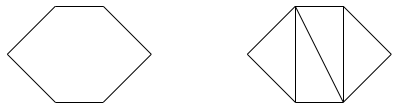
\includegraphics[width=0.5\textwidth]{./Dsa/hex_tri_cells}
   \caption{Discretization using hexagonal cell versus triangle cells}
   \label{fig_hexa_split}
   \end{figure}
 \item \underline{Transition elements and Adaptive Mesh Refinement.} Solvers
   based on arbitrary polyhedral cells can easily handle cells with various
   numbers of edges (2D) and faces (3D). This can be particularly useful for
   simulations with Adaptive Mesh Refinement (AMR)
   \cite{amr_block,amr_rad,amr_unstruc}, without having to deal with the
   implementation of data structures to handle hanging nodes
   \cite{locally_hanging_nodes,arbitrary_hanging_nodes,dealII_hanging_nodes}.
   On Figure \ref{fig_amr}, the left cell is a pentagon whereas the two cells 
   on the right
   are quadrilaterals (a similar illustration can be made for 3D hexahedral
   AMR meshes: suppose a cell is connect to four cells through one of its faces
   - a standard situation with AMR on hexahedral grids - ; such a cell can be
   thought of as a 9-face polyhedron). Thus, a method based on a piecewise linear
   discretization can handle locally adapted meshes without any special
   treatment or further approximation of the coupling between cells.
   \begin{figure}[H]
   \centering
   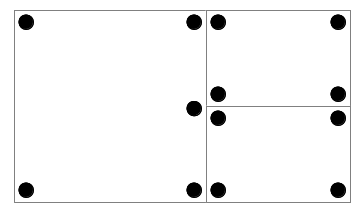
\includegraphics[width=0.3\textwidth]{./Dsa/amr}
   \caption{Example of AMR mesh}
   \label{fig_amr}
   \end{figure}
\end{itemize}
Several discretization methods haven been developed for 
arbitrary polygonal meshes \cite{pwld_3d,pwl_diffusion,pwbld,palmer_fe,mimetic,
cell_centered_diff,palmer_proc,palmer_ane,pwld_2d,wachspress,cfm_dfm}.
In this work, we focus on the PWLD discretization \cite{pwld_3d,pwld_2d}. This
discretization can be applied for any polygonal cells and the integrals
generated by this discretization can be easily computed analytically. 

As of today, a lot of the ongoing effort to develop a DSA scheme on
polygonal/polyhedral cells focuses on adapting the WLA scheme on polygonal meshes
\cite{wla_pwl,cfm_dfm}. The WLA scheme is a two-stage process, where first a
diffusion solution is obtained using a {\em continuous} finite element
discretization and then a {\em discontinuous } update is performed cell-by-cell 
in order to provide an appropriate discontinuous scalar flux to the DFE transport 
solver. In \cite{consistent_p1}, the WLA scheme was
found to be a stable and effective DSA technique, though its efficiency
degraded as the problem became more optically thick and highly diffusive.
To the authors' best knowledge, no work is currently done to adapt the M4S 
technique to polygonal/polyhedral meshes. This is probably due to the fact
that, even though the scheme is effective in one-dimensional slab and
two-dimensional rectangular geometries, it was found to be divergent as an
accelerator for SI in
three-dimensional tetrahedral meshes with linear discontinuous elements.
Furthermore, the scheme does not yield a Symmetric Positive Definite (SPD)
matrix. In this paper, we present an extension of the MIP technique to the
PWLD discretization techniques for for arbitrary polygonal/polyhedral meshes.
The MIP scheme is based on the standard Interior Penalty (IP) for the
discontinuous discretization of diffusion equations. MIP was first derived in
\cite{mip}, where it was applied to triangular unstructured meshes (with
locally adapted cells). MIP did not suffer the degradation of efficiency 
than WLA when the
problem becomes optically thick and highly diffusive and it is therefore an
interesting alternative to WLA. To our knowledge, this work presented the
first DSA scheme based on the same discontinuous trial spaces as the transport
finite element discretization for such meshes. Because MIP produces SPD
equations, it has been solved using conjugate gradient (CG) preconditioned by
a symmetric successive over-relaxation method (SSOR) in \cite{mip}. Here, the
effectiveness of algebraic multigrid methods (AMG) to precondition diffusion
solver \cite{amg,amg_course} will be tested and compared with CG+SSOR.
Algebraic multigrid methods allow the use of multigrid techniques when no grid
information is available or when the grid is unstructured. Instead of using a
succession of grids based on the geometry of the problems, the ``grid levels''
are based on properties of the matrix.
